\documentclass[11pt, a4paper]{article}
\sloppy %prevents text from going over the right margin
% \usepackage[T1]{fontenc}
\usepackage[utf8]{inputenc}
\usepackage{listings}
\usepackage[margin=1.0in]{geometry}
\usepackage{color}
\usepackage{graphicx}
\usepackage{tabularx}
\usepackage{url}
\usepackage[normalem]{ulem} 
\usepackage{enumitem}
\usepackage{hyperref}
\usepackage{fancyhdr} %Package to configure headings and footer
\usepackage{lastpage}
\usepackage[ngerman]{babel}
\setlength\parindent{0pt}

\newcommand{\VARtitle}{NW2}
\newcommand{\VARauthor}{Janeczek}

\title{Meteorologie \\ \VARtitle}
\author{\VARauthor}
\date{\today{}, Vienna}

% header
\pagestyle{fancy}
\fancyhead[L]{\today}
\fancyhead[R]{\VARtitle}

%footer
\fancyfoot[L]{\VARauthor}
\fancyfoot[C]{5AHITT}
\fancyfoot[R]{Page \thepage/\pageref{LastPage}}


\begin{document}

\lstset{ %
  backgroundcolor=\color{white},   % choose the background color; you must add \usepackage{color} or \usepackage{xcolor}
  basicstyle=\footnotesize,        % the size of the fonts that are used for the code
  breakatwhitespace=false,         % sets if automatic breaks should only happen at whitespace
  breaklines=true,                 % sets automatic line breaking
  captionpos=b,                    % sets the caption-position to bottom
% commentstyle=\color{mygreen},    % comment style
  deletekeywords={...},            % if you want to delete keywords from the given language
  escapeinside={\%*}{*)},          % if you want to add LaTeX within your code
  extendedchars=false,              % lets you use non-ASCII characters; for 8-bits encodings only, does not work with UTF-8
% frame=single,                    % adds a frame around the code
  keepspaces=true,                 % keeps spaces in text, useful for keeping indentation of code (possibly needs columns=flexible)
% keywordstyle=\color{blue},       % keyword style
% language=bash,                   % the language of the code
  morekeywords={*,...},            % if you want to add more keywords to the set
  numbers=left,                    % where to put the line-numbers; possible values are (none, left, right)
  numbersep=5pt,                   % how far the line-numbers are from the code
  rulecolor=\color{black},         % if not set, the frame-color may be changed on line-breaks within not-black text (e.g. comments (green here))
  showspaces=false,                % show spaces everywhere adding particular underscores; it overrides 'showstringspaces'
  showstringspaces=false,          % underline spaces within strings only
  showtabs=false,                  % show tabs within strings adding particular underscores
  stepnumber=1,                    % the step between two line-numbers. If it's 1, each line will be numbered
  tabsize=2,                       % sets default tabsize to 2 spaces
  title=\lstname                   % show the filename of files included with \lstinputlisting; also try caption instead of title
}


\maketitle
\newpage
\tableofcontents
\newpage


\section{Vorwort}

In diesem Dokument wird eine meiner naturwissenschaftlichen Thematiken ausgearbeitet. Es handelt sich um den Fachbereich der Meteorologie. Ich werde euch einen wesentlichen Überblick bezüglich der Inversionswetterlage, des Föhns sowie des Golfstroms liefern.

\section{Inversionswetterlage}

\textbf{Was versteht man unter einer sogenannten Inversionswetterlage?}\\
Um näher auf die Inversionswetterlage eingehen zu können, muss der Begriff des \textit{Atmosphärischen Temperaturgradienten} erklärt werden. Prinzipiell befindet sich der atmosphärische Temperaturgradient in der Erdatmosphäre und durch ihn wird beschrieben, wie sehr die Lufttemperatur mit der Höhe zu- oder abnimmt. \\

Durch die Umkehr dieses Temperaturgradienten (lateinisch: inversio), spricht man von einer Inversionswetterlage: Die oberen Luftschichten sind hierbei wärmer als die unteren. \\

In Folge steigt die Lufttemperatur mit der Höhe an, was die Schichtungsstabilität der Troposphäre und insbesondere alle kovektiven Prozesse beeinflusst. Der Bereich, in dem diese Inversion auftritt, wird als Inversionsschicht bezeichnet.\\

Ein Beispiel für eine Inversion lässt sich im Winter beobachten, wenn in klaren Nächsten der Boden auskühlen kann. Dieser kühlt somit auch die unterste Luftschicht, sodass diese stärker abkühlt, als die Luftschichten darüber. Am nächsten Morgen zeigt sich dann bis zur Grenze dieser Schicht der uns bekannte Bodennebel, da die Temperatur der bodennahen Schicht unter den Taupunkt fällt (jener Punkt an dem die relative Luftfeuchtigkeit 100 Prozent beträgt). \\

Aufgrund der höheren Dichte der kälteren Luftschicht, wird die Vermischung mit der darüber liegenden wärmeren Luftschift weitgehend unterdrückt. Die untere Schicht wird also von der oberen abgeschirmt, man spricht von einer stabilen Schichtung. Konvektive Prozesse, beziehungsweise Mechanismen zur Wärmeübertragung von thermischen Energien von einem Ort zu einem anderen, werden verhindert. \\

\begin{figure}[h!]
	\centering
	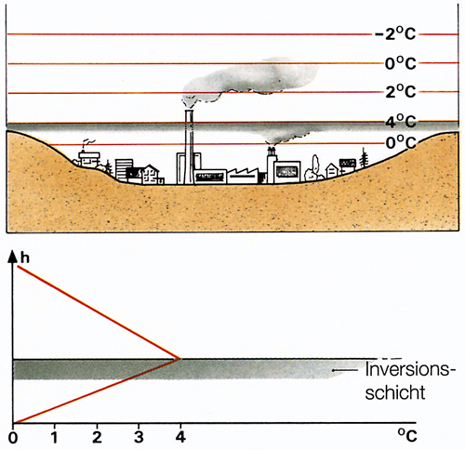
\includegraphics[width=0.5\textwidth]{inversion}
\end{figure}
\newpage
Ein aufsteigendes Luftpaket kühlt sich adiabatisch ab (ohne jeglichen Einfluss von anderen Wärmequellen, es findet kein Wärmeaustausch statt). Da in der Inversionsschicht wärmere Luft oberhalb von kälterer Luft liegt, ist das gerade aufgestiegene Luftpaket schon kälter als seine Umgebung und sinkt daher gleich wieder ab. Der eigentliche Luftaustausch bzw. eine Konvektion ist in der Inversionsschicht nicht möglich. \\

Inversionswetterlagen sorgen auch für geänderte Ausbreitungsbedingungen für Funkwellen. Diese werden am Dichteübergang ins dichtere Medium, hier die kalte Bodenluft totalreflektiert. Es wird gerne von diesem Effekt Gebrauch gemacht, um die Reichweite von Signalen zu erhöhen. Bei UKW (Ultrakurzwellen), die sich im Bereich von 30MHz - 300MHz befinden, kommt es sogar zu Überreichweiten. \\

\textbf{Welche Arten der Bildung einer Inversionswetterlage gibt es?}






\newpage
\nocite{*}
\bibliographystyle{plain}
\bibliography{bibliography}{}

\end{document}